\begin{figure*}%[width=0.75\linewidth]
\begin{center}
\bgroup 
 \def\arraystretch{0.2} 
 \setlength\tabcolsep{0.2pt}
\begin{tabular}{cccccc}
Input & Output & Input & Output & Input & Output \\ 

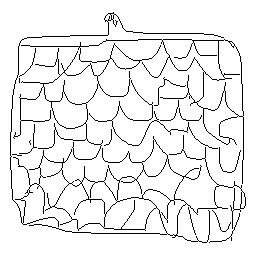
\includegraphics[width=0.167\linewidth]{figs/handbags_sketches_lotsofresults_latex/input_13223.jpg} &
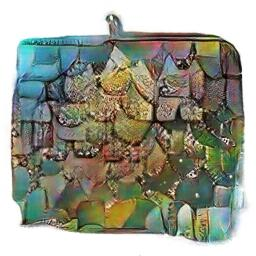
\includegraphics[width=0.167\linewidth]{figs/handbags_sketches_lotsofresults_latex/L1cGAN_13223.jpg} \hspace{0.025in} &
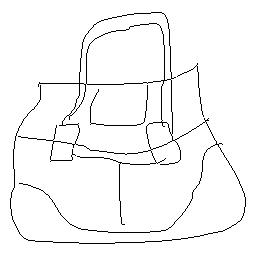
\includegraphics[width=0.167\linewidth]{figs/handbags_sketches_lotsofresults_latex/input_13252.jpg} &
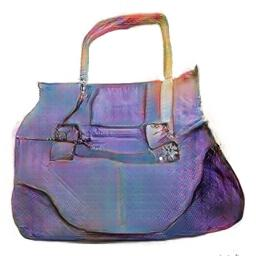
\includegraphics[width=0.167\linewidth]{figs/handbags_sketches_lotsofresults_latex/L1cGAN_13252.jpg} \hspace{0.025in} &

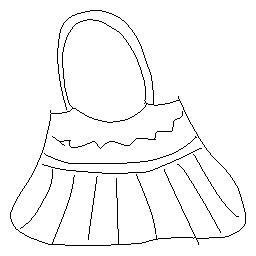
\includegraphics[width=0.167\linewidth]{figs/handbags_sketches_lotsofresults_latex/input_13248.jpg} &
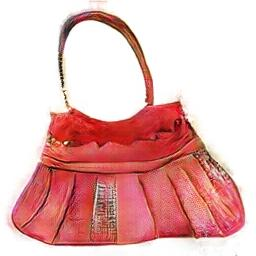
\includegraphics[width=0.167\linewidth]{figs/handbags_sketches_lotsofresults_latex/L1cGAN_13248.jpg} \\
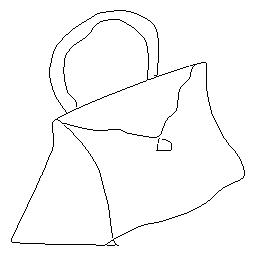
\includegraphics[width=0.167\linewidth]{figs/handbags_sketches_lotsofresults_latex/input_13256.jpg} &
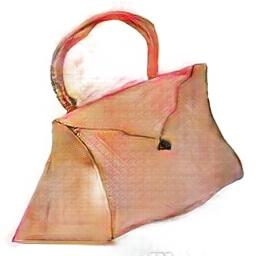
\includegraphics[width=0.167\linewidth]{figs/handbags_sketches_lotsofresults_latex/L1cGAN_13256.jpg} \hspace{0.025in} &

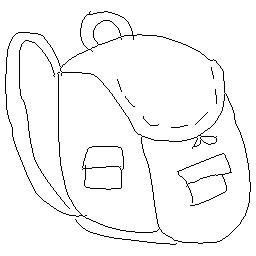
\includegraphics[width=0.167\linewidth]{figs/handbags_sketches_lotsofresults_latex/input_798.jpg} &
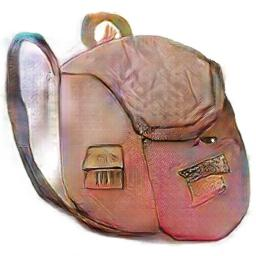
\includegraphics[width=0.167\linewidth]{figs/handbags_sketches_lotsofresults_latex/L1cGAN_798.jpg} \hspace{0.025in} &
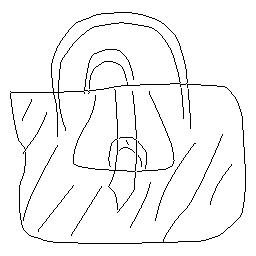
\includegraphics[width=0.167\linewidth]{figs/handbags_sketches_lotsofresults_latex/input_13258.jpg} &
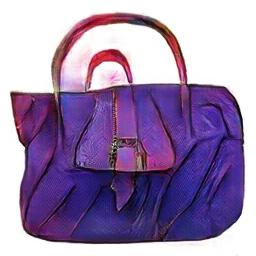
\includegraphics[width=0.167\linewidth]{figs/handbags_sketches_lotsofresults_latex/L1cGAN_13258.jpg} \\

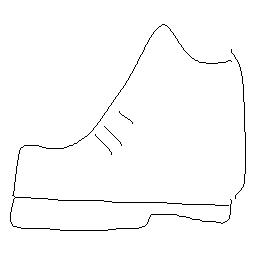
\includegraphics[width=0.167\linewidth]{figs/shoes_sketches_lotsofresults_latex/input_14974.jpg} &
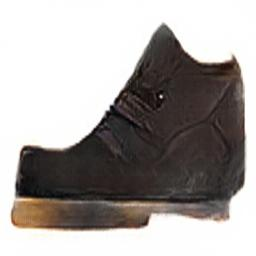
\includegraphics[width=0.167\linewidth]{figs/shoes_sketches_lotsofresults_latex/L1cGAN_14974.jpg} \hspace{0.025in} &
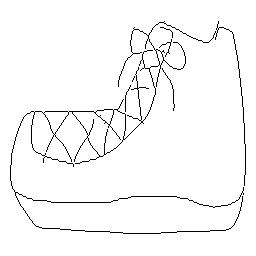
\includegraphics[width=0.167\linewidth]{figs/shoes_sketches_lotsofresults_latex/input_14985.jpg} &
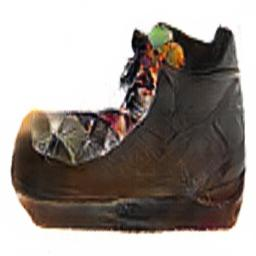
\includegraphics[width=0.167\linewidth]{figs/shoes_sketches_lotsofresults_latex/L1cGAN_14985.jpg} \hspace{0.025in} &

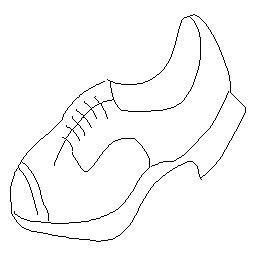
\includegraphics[width=0.167\linewidth]{figs/shoes_sketches_lotsofresults_latex/input_15023.jpg} &
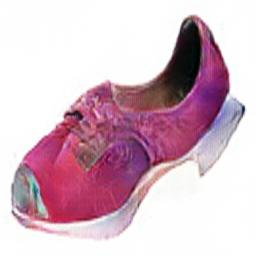
\includegraphics[width=0.167\linewidth]{figs/shoes_sketches_lotsofresults_latex/L1cGAN_15023.jpg} \\
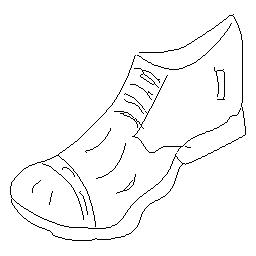
\includegraphics[width=0.167\linewidth]{figs/shoes_sketches_lotsofresults_latex/input_15035.jpg} &
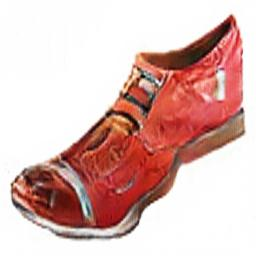
\includegraphics[width=0.167\linewidth]{figs/shoes_sketches_lotsofresults_latex/L1cGAN_15035.jpg} \hspace{0.025in} &

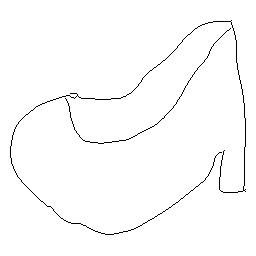
\includegraphics[width=0.167\linewidth]{figs/shoes_sketches_lotsofresults_latex/input_14983.jpg} &
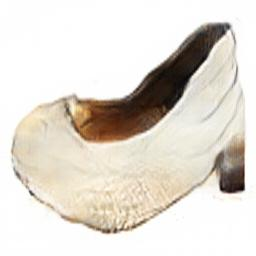
\includegraphics[width=0.167\linewidth]{figs/shoes_sketches_lotsofresults_latex/L1cGAN_14983.jpg} \hspace{0.025in} &
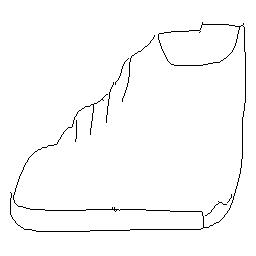
\includegraphics[width=0.167\linewidth]{figs/shoes_sketches_lotsofresults_latex/input_14971.jpg} &
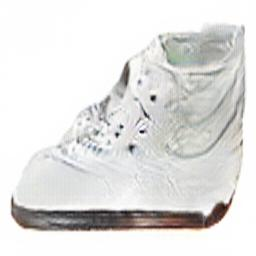
\includegraphics[width=0.167\linewidth]{figs/shoes_sketches_lotsofresults_latex/L1cGAN_14971.jpg}

\end{tabular} \egroup 
\end{center}
\caption{Additional results of the edges$\rightarrow$photo models applied to human-drawn sketches from \cite{eitz2012humans}. Note that the models were trained on automatically detected edges, but generalize to human drawings}
\label{sketches_lotsofresults}
\end{figure*}
